\section{Using cyber contracts to specify security patterns}

The design-by-contract approach \cite{meyer1992applying} states that faults in a software system are the consequence of inadequate programming practices, in contrast to other schools of thought that impute the security problem to even earlier stages of system definition such as requirements elicitation \cite{souag2018Amanda} \cite{mazo2020RSTemplate} \cite{mazo2016framework}and modelling \cite{sun2020domain}. However, this approach was not designed to deal with security issues. Thus, the notion of cyber contract presented in this section, is an extension of the DbC method with concepts coming from the cyber security domain.
In particular, this section (i) formally describes cyber security contracts, (ii) presents the application of such contracts to security patterns, and (iii) develops the case of the authenticator pattern to illustrate our approach.

\subsection{Cyber security contracts}
The core construct of a cyber security contract is the concept of \textit{contract}, which links formal properties and contracting parties as depicted in the  metamodel presented in Figure \ref{fig:CybercontractMetamodel}. The class \textit{Contract} has an attribute \textit{intent}, has a collection of contracting parties and is composed of \textit{Clauses}. The \textit{intent} is a text that describes, in natural language, the purpose of the contract. The contracting parties are represented by the \textit{ContractingParty} class and they correspond to the programming entities whose behaviors are subject to the \textit{Contract}. These entities can be classes, methods, instances, modules, etc. A \textit{Contract}  (i.e., a cyber contract) in our approach differs from the classic view of contracts proposed by Meyer in his DbC paradigm: DbC contracting parties can only be classes and methods whereas ours are not limited by their nature (instances, set of classes, programming units, etc.).. Furthermore, the *-* cardinality in the relation between the \textit{Contract} and \textit{ContractingParty} concepts enables the definition of a \textit{Contract} involving multiple \textit{ContractingParties}, potentially of different nature. This relation also provides the possibility to define multiple contracts for a given \textit{ContractingParty}. In our cyber contract context, the \textit{ContractingParties} stand for the entities involved in the security pattern definition. 

\begin{figure}
    \centering
    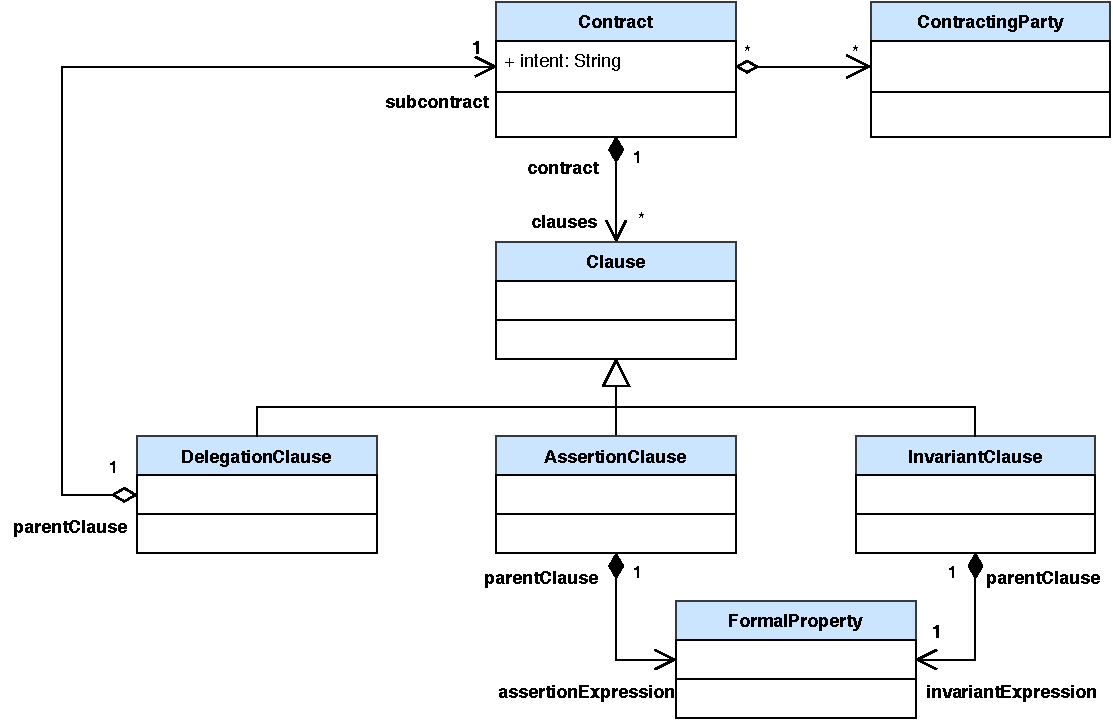
\includegraphics[width=1\columnwidth]{utils/Contract_MM.pdf}
    \caption{Cyber contract metamodel}
    \label{fig:CybercontractMetamodel}
\end{figure}

Every \textit{Contract} is defined as a set of clauses that structure the \textit{FormalProperties} of the corresponding contract \textit{Clauses}. There are three types of \textit{Clauses} that can be added to a \textit{Contract}: \textit{AssertionClause}, \textit{InvariantClause} and \textit{DelegateClause}. 
A \textit{FormalProperty} ensured by the contract refers to one of the two first type of clauses as showed the figure \ref{fig:cybercontractXML} on the Authenticator example.
%The first two clauses wrap a \textit{FormalProperty} which is to be ensured by the contract. 
The \textit{AssertionClauses} enable the specification of assertions that need to be verified at a certain time. They extend the notions of precondition and postcondition of the DbC approach  in a sens that they can be expressed using temporal logic formulas. The \textit{InvariantClauses} are assertions that must always be true, and can therefore be expressed with classical logic. The \textit{DelegateClause} is a concept allowing for responsibilities of a contract to be divided into one or several subcontracts. This mechanism is typically used in the object-oriented paradigm to decompose a contract on the pattern classes, or any decomposition unit of the targeted language.

The last class of the CyberContract metamodel represents the concept of \textit{FormalProperty}. It is an abstraction representing any kind of logic property that one could want to enforce using a contract. In a goal to remain independent of the property expression language, the metamodel does not require any precise expression language.


%Another benefit of our proposal is that a contract can be defined for an assembly of classes, and consequently a security design pattern. Such contract should include all the properties ensuring the correct execution of the pattern. These properties can be functional (i.e., the pattern elements are used in accordance with the pattern description) or implicit  (i.e., a formalization of all implicit meanings of the pattern definition words).

\subsection{Security pattern cybercontract}

Our approach allows for the definition of design pattern contracts. A design pattern is a set of classes and the description of their interactions. We argue that this description can be formalized using a design pattern contract. Such a formalization is particularly relevant regarding security design patterns as presented in Section \ref{PatternLimitations}. 

We have identified two types of formal properties that are relevant to a pattern contract definition: functional and implicit properties.

Functional properties are all the properties expressing the expected behavior of a given pattern. They are the formalization of the interaction of classes as described in the pattern definition. When a pattern is described in natural language, some of the words that are used come with an implicit meaning that can be crucial to the pattern. All these implicit elements, that we call implicit properties, need to be formally expressed in the pattern contract for it to be relevant. A basic example of implicit property is the notion of identifier. Most security design pattern describe fields as identifiers for certain classes. Such identifiers are obviously expected to identify instances of the class. We can for instance define a formal property stating that different instances must have different identifiers. This is an implicit but crucial property.

Thus, as presented in the metamodel, a cyber contract is defined as a set of functional and implicit security properties. The expression of these properties are based on the elements defined in the pattern including classes, instances, attributes and methods. 


\subsection{The Authenticator pattern contract}
\label{label:authenticatorContract}

Let's exemplify the definition of a cybercontract for the Authenticator pattern. To do so, we will use \textit{FormalProperty} expressions based on the object-oriented paradigm for the contract properties.

The \textit{Authenticator} pattern describes a generic authentication mechanism. Six properties have been identified to ensure the security of such a pattern. The first four are implicit properties and the last two are functional properties.
\begin{enumerate}
    \item The first property to check is the uniqueness of the (authentication information, subject) pairs. This property is implicit in the pattern definition but is fundamental. Indeed, if it is not verified, the pattern has no more meaning since an \textit{authentication information} would not identify a unique subject. With $I_{Subject}$ containing all instances of the $Subject$ class, the property can be expressed as follows.
    \begin{equation*}
        P1: \forall a, b \in I_{Subject}, a \ne b \implies a.authInfo \ne b.authInfo
    \end{equation*}
    \item Similarly, since the authentication information is linked to the subject instance, it must not vary during execution (probable identity theft). Let $a.authInfo_{ini}$ be the initial value of the field $authInfo$ of the $Subject$ instance $a$. Formally:
    \begin{equation*}
        P2: \forall a \in I_{Subject}, a.authInfo = a.authInfo_{ini}
    \end{equation*}
    \item A major flaw that can jeopardize authentication systems concerns the non-integrity of the authentication authority. In order to be authenticated, a subject must make a request to the Authenticator. If an attacker succeeds in forging its Authenticator, he becomes master of the authentication system. It is therefore essential that the Authenticator cannot be modified. Thus, let  $a.authenticator_{ini}$ be the initial value of the field $authenticator$ of the $Subject$ instance $a$. This property can then be expressed as follows.
    \begin{equation*}
        P3: \forall a \in I_{Subject}, a.authenticator = a.authenticator_{ini}
    \end{equation*}
    \item At all time, the proof of identity of every subject must be either valid or undefined.
    \begin{equation*}
    \begin{split}
        &P4: \forall a \in I_{Subject}, (a.idProof = \emptyset) \lor \\&(a.idProof = a.authenticator.request(a.authInfo))
    \end{split}
    \end{equation*}
    \item After authentication, the proof of identity must be the one returned by the request method with the correct parameters. According to the DbC approach, it means that the following property should be ensured by the \textit{authenticate} method of the \textit{Subject} class.
    \begin{equation*}
        P5: self.idProof = self.authenticator.request(self.authInfo)
    \end{equation*}
%    \item 
    \item The proof of identity returned by the \textit{request} method of the \textit{Authenticator} class must be valid if and only if the subject requesting it is who it claims to be. More formally, it means that the \textit{request} method must ensure the following property. Let $\emptyset$ be the default value for a variable. The postcondition can then be expressed as follows.
    \begin{equation*}
        P6: self.check(authInfo) \lor returnValue = \emptyset
    \end{equation*}
\end{enumerate}

Figure \ref{fig:cybercontractXML} shows a simplified XML representation of this contract.
This representation illustrates an instantiation of our metamodel on the Authenticator cyber contract. The binding with the Authenticator pattern is explicit and we can see the property P1 as an \textit{InvariantClause} defined at the pattern scope.
The delegation mechanism provided with the \textit{DelegateClauses} is also illustrated within this example. Some of the previous properties are indeed within the scope of a single method (P5 and P6). They are thus delegated to the relevant classes using a \textit{DelegateClause} (keyword \textit{Subcontract}) and then to the correct methods.

%For example purposes, let's consider one possible expression language for the \textit{FormalProperty} concept, base on the object-oriented paradigm. This expression language will then be used to define the cybercontract of the Authenticator pattern, described with the object-oriented paradigm.
%si j'ai bien compris, ce qu'on a voulu faire ici c'est de présenter un exemple de l'utilisation de ce concept dans le cas du Authentication patten. Si c'est cela voici comme on dévrait présenter la chose:
%Let's show the implementation of a proof of concept for the \textit{FormalProperty} class. To do so, let's consider the Authenticator pattern, implemented in an object-oriented language, to represent the formal properties corresponding to its CyberContract.
%et ensuite on présente tout ce qu'il y a dans la section Authenticator CyberContract (sans être une section mais comme une continuation de cette sub-section) et la partie $I_{Class}$, $var_{ini}$ et $\emptyset$ on la présente au moment de l'utilisation de chaque concept avec un Where $\emptyset$ represents  the... car avec la manière comme on est en train de présenter la chose on les oublie tout de suite et ça fait revenir le lecteur pour consulter la def de chaque chose et cela est très genant.
%Let's consider the following notations for the properties:
%\begin{itemize}
%    \item Let $I_{Class}$ be the set containing all instances of the class $Class$.
%    \item Let $var_{ini}$ be the initial value (right after the constructor call) of the variable $var$.
%    \item Let $\emptyset$ be the undefined state for a variable.
%\end{itemize}
%As for the logic system of the properties, the contract \textit{Boolean expressions} use the mathematical operators $\forall$ and $\exists$ along with classical Boolean operators ($\implies$, $\land$, etc.).

%Let's now consider the  Authenticator pattern 

%ici il faut préparer le lecteur à la section suivante car le changement est très abrupt (je vais lire la section pour savoir ce qu'elle présente et voir si je peux faire ici le lien)

\begin{figure}
    \centering
 \begin{lstlisting}[breaklines=true, language=XML, basicstyle=\ttfamily\footnotesize, mathescape=true]
<Contract>
    <binding "Authenticator_pattern" />  
    <clauses> 
    <InvariantClause P1/>  
    <Subcontract "SubjectContract">
        <binding "Subject" />
        <InvariantClause P2 $\land$ P3 $\land$ P4/>
        <Subcontract "authenticateContract"s>
            <binding "void authenticate()">
            <ensures P5/>
        </Subcontract>
    </Subcontract>
    <Subcontract "AuthenticatorContract">
        <binding "Authenticator"/>
        <Subcontract "requestContract">
            <binding = "ProofOfIdentity request(AuthenticationInformation authInfo)">
            <ensures P6/>
        </Subcontract>
    </Subcontract>
    </clauses>
</Contract>

\end{lstlisting}
\begin{equation}
\begin{split}
\\
&P1: \forall a, b \in I_{Subject},a \ne b \implies a.authInfo \ne b.authInfo\\
&P2: \forall a \in I_{Subject}, a.authInfo = a.authInfo_{ini}\\
&P3: \forall a \in I_{Subject}, a.authenticator = a. authenticator_{ini}\\
&P4: \forall a \in I_{Subject}, a.idProof = \emptyset \lor \\
&a.idProof = authenticator.request(authInfo)\\
&P5: self.idProof = self.authenticator.request(self.authInfo)\\
&P6: self.check(authInfo) \lor returnValue = \emptyset
\end{split}
\nonumber
\end{equation}
\caption{XML representation of the Authenticator pattern contract}
\label{fig:cybercontractXML}
\end{figure}